\documentclass[border=8pt]{standalone}
\usepackage[T1]{fontenc}\usepackage{helvet}\renewcommand{\familydefault}{\sfdefault}
\usepackage{tikz}\usetikzlibrary{arrows.meta, positioning, calc, backgrounds}
\definecolor{ink}{HTML}{1a1916}
\definecolor{inktwo}{HTML}{3a3a35}
\definecolor{inkthree}{HTML}{6a6862}
\definecolor{rule}{HTML}{b8b09a}
\definecolor{amber}{HTML}{a8730a}
\definecolor{red}{HTML}{c8261a}
\definecolor{paper}{HTML}{f0eee5}
\definecolor{slab}{HTML}{d8d4c6}
\tikzset{
  >={Stealth[length=2.2mm]},
  wire/.style={line width=0.8pt, ink},
  modwire/.style={line width=0.6pt, dashed, ink},
  tastewire/.style={line width=0.6pt, dashed, amber},
  gatewire/.style={line width=0.6pt, dotted, ink},
  block/.style={rectangle, draw=ink, line width=0.9pt, fill=slab, minimum width=3.0cm, minimum height=1.9cm, inner sep=0pt},
  perf/.style={rectangle, draw=ink, line width=0.7pt, minimum width=3.0cm, minimum height=0.7cm, inner sep=2pt, font=\footnotesize, text=ink},
  title/.style={font=\scriptsize\bfseries, text=ink, anchor=north, inner sep=2pt},
  jack/.style={circle, draw=ink, fill=paper, line width=0.5pt, minimum size=3.2pt, inner sep=0pt},
  plabel/.style={font=\tiny, text=inktwo, anchor=west, inner sep=1pt},
  olabel/.style={font=\tiny, text=inktwo, anchor=east, inner sep=1pt},
  settings/.style={font=\scriptsize, text=ink, align=left, anchor=north west, inner sep=1pt, text width=2.9cm},
}
\begin{document}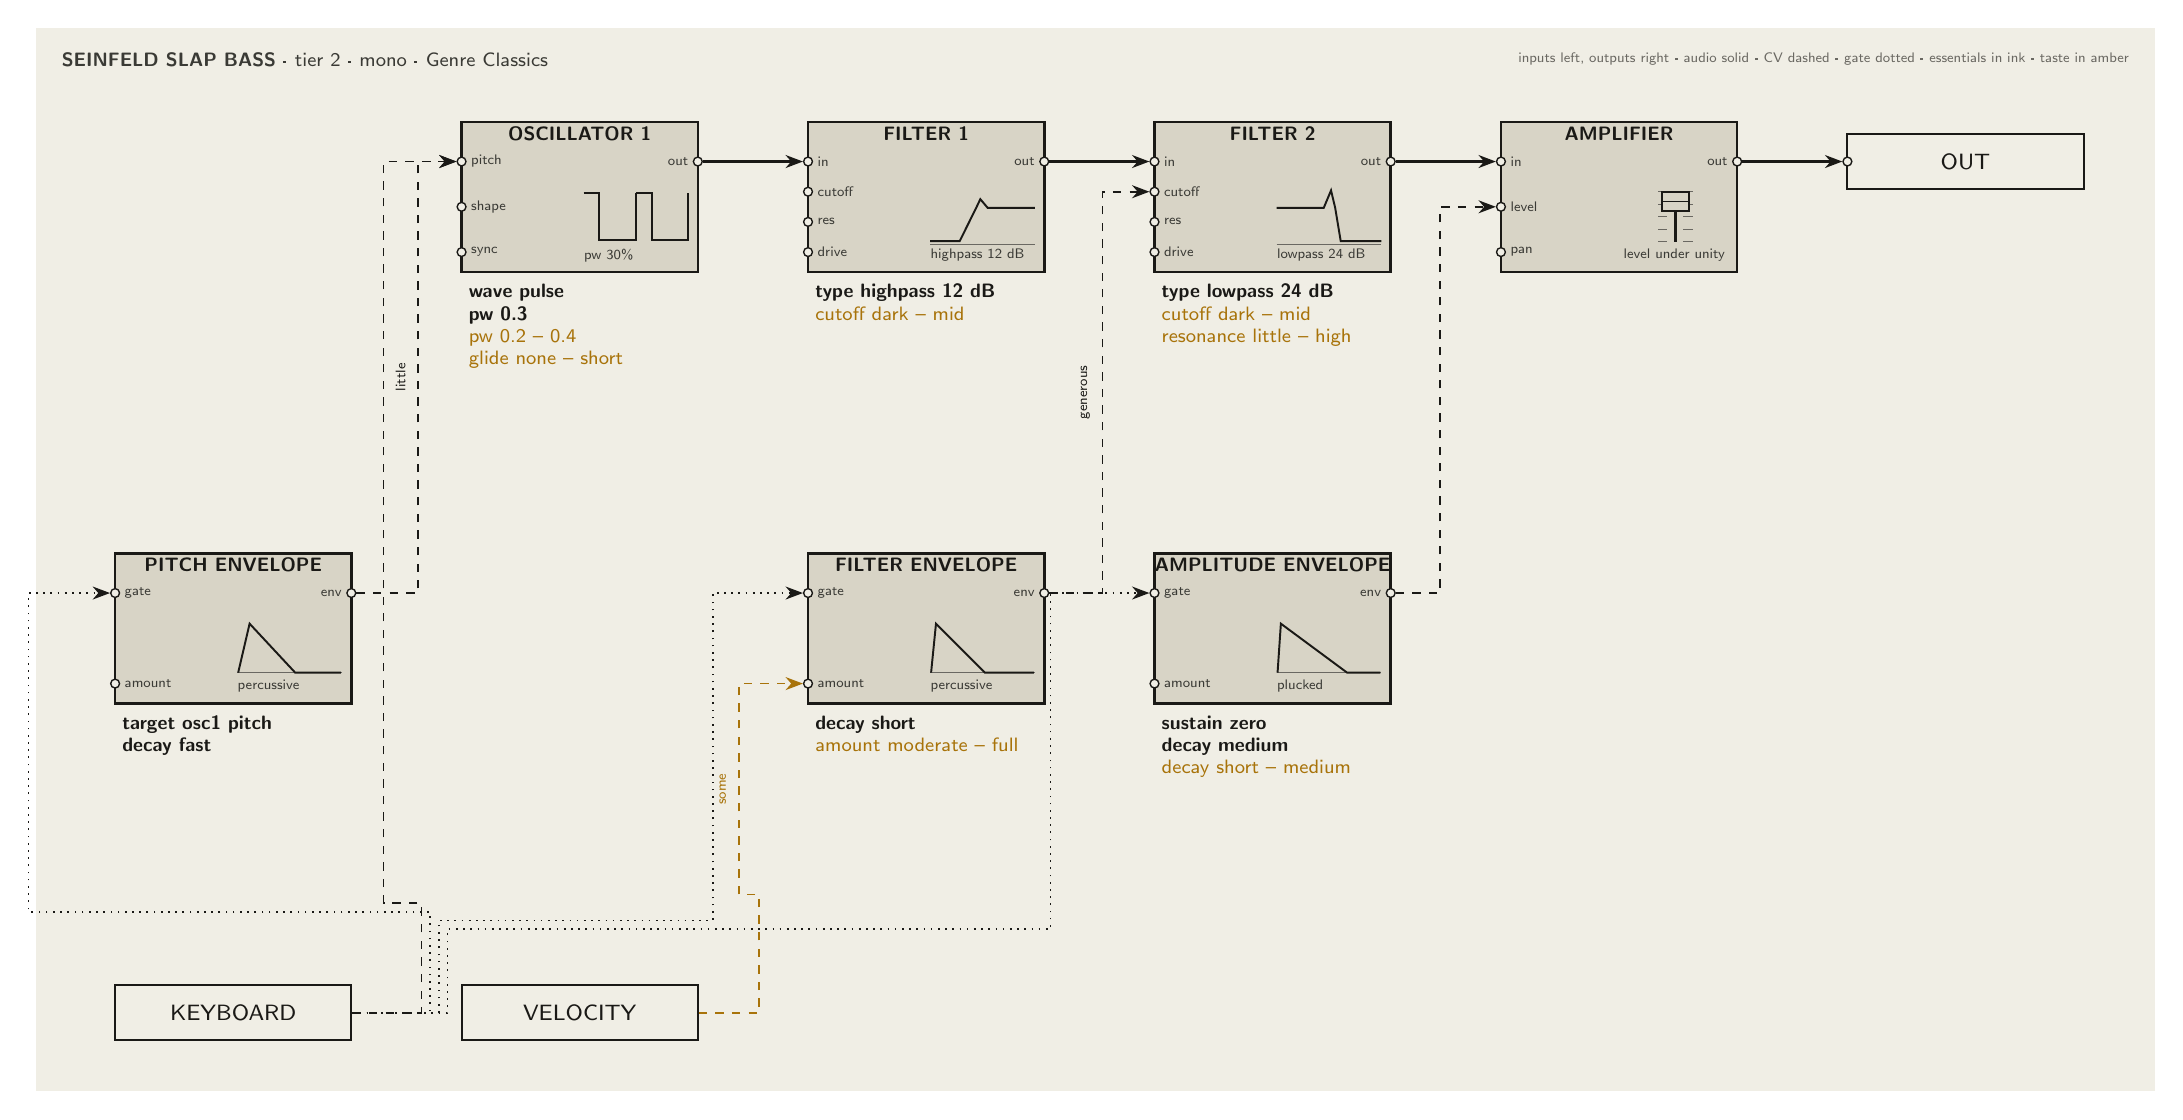
\begin{tikzpicture}
\begin{scope}[on background layer]\fill[paper] (-2.5,-11.36) rectangle (24.4,2.15);\end{scope}
\node[block, minimum height=1.9cm] (osc1) at (4.4,0.0) {};
\node[title] at (osc1.north) {OSCILLATOR 1};
\node[jack] (osc1-pitch) at (2.9000000000000004,0.44999999999999996) {};
\node[plabel] at (2.9800000000000004,0.44999999999999996) {pitch};
\node[jack] (osc1-shape) at (2.9000000000000004,-0.125) {};
\node[plabel] at (2.9800000000000004,-0.125) {shape};
\node[jack] (osc1-sync) at (2.9000000000000004,-0.7) {};
\node[plabel] at (2.9800000000000004,-0.7) {sync};
\node[jack] (osc1-out) at (5.9,0.44999999999999996) {};
\node[olabel] at (5.82,0.44999999999999996) {out};
\begin{scope}
\draw[ink, line width=0.7pt] (4.450,0.046) -- (4.649,0.046) -- (4.649,-0.546) -- (5.115,-0.546) -- (5.115,0.046);
\draw[ink, line width=0.7pt] (5.115,0.046) -- (5.315,0.046) -- (5.315,-0.546) -- (5.780,-0.546) -- (5.780,0.046);
\node[font=\tiny, text=inktwo, anchor=north west, inner sep=0pt] at (4.450,-0.650) {pw 30\%};
\end{scope}
\node[settings] at (2.95,-1.0699999999999998) {\textbf{wave pulse} \\ \textbf{pw 0.3} \\ \textcolor{amber}{pw 0.2 -- 0.4} \\ \textcolor{amber}{glide none -- short}};
\node[block, minimum height=1.9cm] (filter1) at (8.8,0.0) {};
\node[title] at (filter1.north) {FILTER 1};
\node[jack] (filter1-in) at (7.300000000000001,0.44999999999999996) {};
\node[plabel] at (7.380000000000001,0.44999999999999996) {in};
\node[jack] (filter1-cutoff) at (7.300000000000001,0.06666666666666665) {};
\node[plabel] at (7.380000000000001,0.06666666666666665) {cutoff};
\node[jack] (filter1-res) at (7.300000000000001,-0.31666666666666665) {};
\node[plabel] at (7.380000000000001,-0.31666666666666665) {res};
\node[jack] (filter1-drive) at (7.300000000000001,-0.7) {};
\node[plabel] at (7.380000000000001,-0.7) {drive};
\node[jack] (filter1-out) at (10.3,0.44999999999999996) {};
\node[olabel] at (10.22,0.44999999999999996) {out};
\begin{scope}
\draw[inkthree, line width=0.3pt] (8.850,-0.605) -- (10.180,-0.605);
\draw[ink, line width=0.7pt] (8.850,-0.561) -- (9.226,-0.561) -- (9.435,-0.139) -- (9.488,-0.028) -- (9.582,-0.139) -- (10.180,-0.139);
\node[font=\tiny, text=inktwo, anchor=north west, inner sep=0pt] at (8.850,-0.650) {highpass 12 dB};
\end{scope}
\node[settings] at (7.3500000000000005,-1.0699999999999998) {\textbf{type highpass 12 dB} \\ \textcolor{amber}{cutoff dark -- mid}};
\node[block, minimum height=1.9cm] (filter2) at (13.200000000000001,0.0) {};
\node[title] at (filter2.north) {FILTER 2};
\node[jack] (filter2-in) at (11.700000000000001,0.44999999999999996) {};
\node[plabel] at (11.780000000000001,0.44999999999999996) {in};
\node[jack] (filter2-cutoff) at (11.700000000000001,0.06666666666666665) {};
\node[plabel] at (11.780000000000001,0.06666666666666665) {cutoff};
\node[jack] (filter2-res) at (11.700000000000001,-0.31666666666666665) {};
\node[plabel] at (11.780000000000001,-0.31666666666666665) {res};
\node[jack] (filter2-drive) at (11.700000000000001,-0.7) {};
\node[plabel] at (11.780000000000001,-0.7) {drive};
\node[jack] (filter2-out) at (14.700000000000001,0.44999999999999996) {};
\node[olabel] at (14.620000000000001,0.44999999999999996) {out};
\begin{scope}
\draw[inkthree, line width=0.3pt] (13.250,-0.605) -- (14.580,-0.605);
\draw[ink, line width=0.7pt] (13.250,-0.139) -- (13.849,-0.139) -- (13.942,0.083) -- (13.995,-0.139) -- (14.065,-0.561) -- (14.580,-0.561);
\node[font=\tiny, text=inktwo, anchor=north west, inner sep=0pt] at (13.250,-0.650) {lowpass 24 dB};
\end{scope}
\node[settings] at (11.750000000000002,-1.0699999999999998) {\textbf{type lowpass 24 dB} \\ \textcolor{amber}{cutoff dark -- mid} \\ \textcolor{amber}{resonance little -- high}};
\node[block, minimum height=1.9cm] (amp) at (17.6,0.0) {};
\node[title] at (amp.north) {AMPLIFIER};
\node[jack] (amp-in) at (16.1,0.44999999999999996) {};
\node[plabel] at (16.18,0.44999999999999996) {in};
\node[jack] (amp-level) at (16.1,-0.125) {};
\node[plabel] at (16.18,-0.125) {level};
\node[jack] (amp-pan) at (16.1,-0.7) {};
\node[plabel] at (16.18,-0.7) {pan};
\node[jack] (amp-out) at (19.1,0.44999999999999996) {};
\node[olabel] at (19.020000000000003,0.44999999999999996) {out};
\begin{scope}
\draw[ink, line width=1.2pt] (18.315,-0.570) -- (18.315,0.070);
\draw[inkthree, line width=0.3pt] (18.095,-0.570) -- (18.215,-0.570) (18.415,-0.570) -- (18.535,-0.570);
\draw[inkthree, line width=0.3pt] (18.095,-0.410) -- (18.215,-0.410) (18.415,-0.410) -- (18.535,-0.410);
\draw[inkthree, line width=0.3pt] (18.095,-0.250) -- (18.215,-0.250) (18.415,-0.250) -- (18.535,-0.250);
\draw[inkthree, line width=0.3pt] (18.095,-0.090) -- (18.215,-0.090) (18.415,-0.090) -- (18.535,-0.090);
\draw[inkthree, line width=0.3pt] (18.095,0.070) -- (18.215,0.070) (18.415,0.070) -- (18.535,0.070);
\fill[slab, draw=ink, line width=0.6pt] (18.145,-0.178) rectangle (18.485,0.062);
\draw[ink, line width=0.5pt] (18.145,-0.058) -- (18.485,-0.058);
\node[font=\tiny, text=inktwo, anchor=north west, inner sep=0pt] at (17.650,-0.650) {level under unity};
\end{scope}
\node[block, minimum height=1.9cm] (menv) at (0.0,-5.4799999999999995) {};
\node[title] at (menv.north) {PITCH ENVELOPE};
\node[jack] (menv-gate) at (-1.5,-5.029999999999999) {};
\node[plabel] at (-1.42,-5.029999999999999) {gate};
\node[jack] (menv-amount) at (-1.5,-6.18) {};
\node[plabel] at (-1.42,-6.18) {amount};
\node[jack] (menv-out) at (1.5,-5.029999999999999) {};
\node[olabel] at (1.42,-5.029999999999999) {env};
\begin{scope}
\draw[inkthree, line width=0.3pt] (0.050,-6.041) -- (1.380,-6.041);
\draw[ink, line width=0.7pt] (0.063,-6.041) -- (0.208,-5.419) -- (0.787,-6.041) -- (0.787,-6.041) -- (1.367,-6.041);
\node[font=\tiny, text=inktwo, anchor=north west, inner sep=0pt] at (0.050,-6.130) {percussive};
\end{scope}
\node[settings] at (-1.45,-6.55) {\textbf{target osc1 pitch} \\ \textbf{decay fast}};
\node[block, minimum height=1.9cm] (fenv) at (8.8,-5.4799999999999995) {};
\node[title] at (fenv.north) {FILTER ENVELOPE};
\node[jack] (fenv-gate) at (7.300000000000001,-5.029999999999999) {};
\node[plabel] at (7.380000000000001,-5.029999999999999) {gate};
\node[jack] (fenv-amount) at (7.300000000000001,-6.18) {};
\node[plabel] at (7.380000000000001,-6.18) {amount};
\node[jack] (fenv-out) at (10.3,-5.029999999999999) {};
\node[olabel] at (10.22,-5.029999999999999) {env};
\begin{scope}
\draw[inkthree, line width=0.3pt] (8.850,-6.041) -- (10.180,-6.041);
\draw[ink, line width=0.7pt] (8.863,-6.041) -- (8.925,-5.419) -- (9.546,-6.041) -- (9.546,-6.041) -- (10.167,-6.041);
\node[font=\tiny, text=inktwo, anchor=north west, inner sep=0pt] at (8.850,-6.130) {percussive};
\end{scope}
\node[settings] at (7.3500000000000005,-6.55) {\textbf{decay short} \\ \textcolor{amber}{amount moderate -- full}};
\node[block, minimum height=1.9cm] (aenv) at (13.200000000000001,-5.4799999999999995) {};
\node[title] at (aenv.north) {AMPLITUDE ENVELOPE};
\node[jack] (aenv-gate) at (11.700000000000001,-5.029999999999999) {};
\node[plabel] at (11.780000000000001,-5.029999999999999) {gate};
\node[jack] (aenv-amount) at (11.700000000000001,-6.18) {};
\node[plabel] at (11.780000000000001,-6.18) {amount};
\node[jack] (aenv-out) at (14.700000000000001,-5.029999999999999) {};
\node[olabel] at (14.620000000000001,-5.029999999999999) {env};
\begin{scope}
\draw[inkthree, line width=0.3pt] (13.250,-6.041) -- (14.580,-6.041);
\draw[ink, line width=0.7pt] (13.263,-6.041) -- (13.305,-5.419) -- (14.146,-6.041) -- (14.146,-6.041) -- (14.567,-6.041);
\node[font=\tiny, text=inktwo, anchor=north west, inner sep=0pt] at (13.250,-6.130) {plucked};
\end{scope}
\node[settings] at (11.750000000000002,-6.55) {\textbf{sustain zero} \\ \textbf{decay medium} \\ \textcolor{amber}{decay short -- medium}};
\node[perf] (key) at (0.0,-10.36) {KEYBOARD};
\node[perf] (vel) at (4.4,-10.36) {VELOCITY};
\node[perf, fill=paper] (out) at (22.0,0.44999999999999996) {OUT}; \node[jack] (out-in) at (20.5,0.44999999999999996) {};
\draw[wire,->] (osc1-out) -- (filter1-in);
\draw[wire,->] (filter1-out) -- (filter2-in);
\draw[wire,->] (filter2-out) -- (amp-in);
\draw[wire,->] (amp-out) -- (out-in);
\draw[modwire,->] (menv-out) -- (2.3500000000000005,-5.029999999999999) -- (2.3500000000000005,0.44999999999999996) -- (osc1-pitch);
\node[font=\tiny, text=ink, anchor=south, inner sep=1pt, rotate=90] at (2.2300000000000004,-2.2899999999999996) {little};
\draw[modwire,->] (fenv-out) -- (11.040000000000001,-5.029999999999999) -- (11.040000000000001,0.06666666666666665) -- (filter2-cutoff);
\node[font=\tiny, text=ink, anchor=south, inner sep=1pt, rotate=90] at (10.920000000000002,-2.4816666666666665) {generous};
\draw[modwire,->] (aenv-out) -- (15.33,-5.029999999999999) -- (15.33,-0.125) -- (amp-level);
\draw[tastewire,->] (vel.east) -- (6.680000000000001,-10.36) -- (6.680000000000001,-8.86) -- (6.420000000000001,-8.86) -- (6.420000000000001,-6.18) -- (fenv-amount);
\node[font=\tiny, text=amber, anchor=south, inner sep=1pt, rotate=90] at (6.300000000000001,-7.52) {some};
\draw[modwire,->] (key.east) -- (2.39,-10.36) -- (2.39,-8.969999999999999) -- (1.9100000000000006,-8.969999999999999) -- (1.9100000000000006,0.44999999999999996) -- (osc1-pitch);
\draw[gatewire,->] (key.east) -- (2.5,-10.36) -- (2.5,-9.08) -- (-2.5999999999999996,-9.08) -- (-2.5999999999999996,-5.029999999999999) -- (menv-gate);
\draw[gatewire,->] (key.east) -- (2.61,-10.36) -- (2.61,-9.19) -- (6.090000000000001,-9.19) -- (6.090000000000001,-5.029999999999999) -- (fenv-gate);
\draw[gatewire,->] (key.east) -- (2.7199999999999998,-10.36) -- (2.7199999999999998,-9.299999999999999) -- (10.38,-9.299999999999999) -- (10.38,-5.029999999999999) -- (aenv-gate);
\node[anchor=north west, font=\scriptsize, text=inktwo] at (-2.3,1.95) {\textbf{SEINFELD SLAP BASS} · tier 2 · mono · Genre Classics};
\node[anchor=north east, font=\tiny, text=inkthree] at (24.2,1.95) {inputs left, outputs right · audio solid · CV dashed · gate dotted · essentials in ink · taste in amber};
\end{tikzpicture}\end{document}
